\label{sec:vst}

%\marginpar{\tiny \color{blue} These brief explanations of VST and Floyd need to come in much earlier...}
CompCert is a fully machine-checked verified compiler for~CompCert C~\cite{leroy:compcert}.
The Verified Software Toolchain consists of a series of machine-checked modules written in Coq
to reason about CompCert C programs~\cite{appel:programlogics}.
Floyd is VST's module for verifying such programs using separation logic.
VST's modules interlock so there are no ``gaps'' in the end-to-end certified results;
accordingly all of the rules employed by Floyd have been proved sound with respect to
the underlying semantics used by CompCert.  Floyd is written in Ltac and Gallina and is
designed to help users verify the full functional correctness of their programs.
We added two tactics, \li{localize} and \li{unlocalize}, to
integrate the \textsc{Localize} rule into Floyd as described in \S\ref{sec:orientation}--\S\ref{sec:localizations}.


%Although Floyd devotes considerable effort to make this task simpler, it prefers expressibility and completeness to more automated tools like HIP/SLEEK.


\subsection{Localizations in VST with \li{localize} and \li{unlocalize}}
\label{sec:vstlocalunlocal}
\vspace{-0.75ex}
Floyd presents users with a pleasant ``decorated program'' visualization for Hoare proofs, in which users work from the top of the program to the bottom even though the formal proof is maintained as applications of inference rules.  For example, suppose the proof goal is $\triple{P_1}{c_1\li{;}c_2}{P_5}$ and VST's user tells Floyd to apply a Hoare rule for $c_1$, \emph{e.g.}~$\triple{P_1}{c_1}{P_2}$.  Floyd will then automatically apply the \infrulestyle{Sequence} rule and show the user $\triple{P_2}{c_2}{P_5}$ as the remaining goal.
When the user is in the middle of a verification, the decorated program is partially done (\emph{i.e.} the proof is finished from the top to ``the current program point'') and the inference tree is also partially done (\emph{i.e.} with holes that are represented by the remaining proof goals in Coq).

We wish to preserve this ``decorated program'' view while extending Floyd to support localization.  Our task therefore is to construct a proof in Coq's underlying logic that allows a localization block to be constructed in this manner---that is, we wish to enter a localization block without requiring the user to specify the ``exit point'' in advance.  The engineering is tricky because the proof Floyd is constructing (\emph{i.e.} applications of inference rules) has holes in places where the user's ``top to bottom'' view of things has not yet arrived.

%\begin{wrapfigure}{l}{.63\textwidth}
\begin{figure}
\begin{minipage}{.15\textwidth}
\begin{lstlisting}[basicstyle=\linespread{0.8}\normalfont\footnotesize\tt]
$\{\ \ P_1 \ \ \}$
    c1
$\{\ \ P_2 \ \ \}\label{code:localglobalin}$
$\searrow \{\ \ P_3 \ \ \}\label{code:locallocalin}$
      c2;
  $\,\{\ \ P_4 \ \ \}\label{code:localsndcmd}$

    ...


\end{lstlisting}
\centerline{\footnotesize(front)}
\end{minipage} \vline ~
\begin{minipage}{.15\textwidth}
\begin{lstlisting}[numbers=none, basicstyle=\linespread{0.8}\normalfont\footnotesize\tt]
$\{\ \ P_1 \ \ \}$
    c1
$\{\ \ P_2 \ \ \}$
$\{\ \ ?F * P_3 \ \}$
    c2;
$\{\ \ ?F * P_4 \ \}$

  ...


\end{lstlisting}
\centerline{\footnotesize(back)}
\end{minipage} \vline \vline ~
\begin{minipage}{.15\textwidth}
\begin{lstlisting}[numbers=none, basicstyle=\linespread{0.8}\normalfont\footnotesize\tt]
$\{\ \ P_1 \ \ \}$
    c1
$\{\ \ P_2 \ \ \}$
$\searrow \{\ \ P_3 \ \ \}$
      c2;
  $\,\{\ \ P_4 \ \ \}$
      c3;
$\swarrow\{\ \ P_5 \ \ \}$
$\{\ \ P_6 \ \ \}$
    ...
\end{lstlisting}
\centerline{\footnotesize(front)}
\end{minipage} \vline ~
\begin{minipage}{.15\textwidth}
\begin{lstlisting}[numbers=none, basicstyle=\linespread{0.8}\normalfont\footnotesize\tt]
$\{\ \ P_1 \ \ \}$
    c1
$\{\ \ P_2 \ \ \}$
$\{\ \ ?F * P_3 \ \}$
    c2;
$\{\ \ ?F * P_4 \ \}$
    c3;
$\{\ \ ?F * P_5 \ \}$
$\{\ \ P_6 \ \ \}$
  ...
\end{lstlisting}
\centerline{\footnotesize(back)}
\end{minipage}
%\vspace{-ex}
\caption{Front and back ends of \li{localize} and \li{unlocalize}}
\label{figure:backend}
\end{figure}
%\end{wrapfigure}

Figure~\ref{figure:backend} has two partially-decorated ``proofs in progress'', from both the user's (front end) and Floyd's (back end) points of view.  In the first column, from the user's point of view, they saw the assertion $P_2$ (line~\ref{code:localglobalin}) and decided to use the \li{localize} tactic to zoom into $P_3$ (line~\ref{code:locallocalin}).  They then applied some proof rules to move past $c_2$ to reach the assertion $P_4$ (line~\ref{code:localsndcmd}).  At this point, Floyd does not know when the corresponding \li{unlocalize} tactic will execute, so it does not know which commands will be inside the block or what the final local and global postconditions will be.

Accordingly, the \li{localize} tactic builds an incremental proof in the underlying program logic by applying \infrulestyle{Frame} with an uninstantiated metavariable.
The second column of Figure~\ref{figure:backend} shows the back end with the unknown frame $?F$, which will eventually be instantiated by \li{unlocalize}.

In the third column, the user has advanced past $c_3$ to reach the local postcondition $P_5$ and now wishes to \li{unlocalize} to~$P_6$.  Afterwards, the internal state looks like the fourth column, and so to a first approximation, \li{unlocalize} can instantiate $?F$ with $P_5 \wand P_6$.  In truth, $?F$ is chosen more subtly to properly handle both existential variables and modified program variables; \li{unlocalize} then automatically simplifies the goals to present a cleaner interface to the user.  These transformations require the additional theory given in \S\ref{sec:localizations}.


\subsection{Statistics related to our development}

\begin{table}[b]
\centering
\begin{tabular}{c|c|c|c|c|c}
Component & Section & Files & Size (in lines) & Definitions & Theorems\\\hline
Common Utilities & & 10 & 3,578 & 44 & 289 \\
Math Graph Library & \S\ref{sec:mathgraph} & 20 & 10,585 & 216 & 581 \\
Spatial Graph Library & \S\ref{sec:spacegraph} & 3 & 2,328 & 59 & 110 \\
Integration into VST & \S\ref{sec:localizations},\S\ref{sec:development} & 11 & 2,783 & 17 & 172 \\
\hline
Marking (graph and DAG) & \S\ref{sec:localizations} & 6 & 775 & 9 & 20 \\
Spanning Tree & \S\ref{sec:localizations} & 5 & 2,723 & 17 & 92 \\
Union-Find (heap and array) & \S\ref{sec:orientation} & 18 & 3,193 & 107 & 135 \\
Garbage Collector & \S\ref{sec:certigc} & 16 & 13,858 & 235 & 712 \\
\hline & & & & & \\
[-2.2em] \\
\hline & & & & & \\
[-1em]
Total Development & & 89 & 39,823 & 704 & 2,111 \\
\end{tabular}
\caption{Statistics for our code base}
\label{tab:codebase}
\end{table}

All our results in this paper have been machine-checked.
%The bulk of our development was checked in Coq, although a 55-line file (shown in Figure~\ref{fig:hipmarkgraph}) was checked in HIP/SLEEK.  Our modifications to H/S itself were not machine-checked since H/S does not have a mechanized soundness proof.
Although the size of a development does not perfectly match that development's 
importance or the difficulty of its implementation, 
we present the size nonetheless in Table~\ref{tab:codebase}.
%, organized roughly by the paper section corresponding to each development.
Our proof script is written in a very
dense style.
For comparison, verifying a simple 39-line list-based merge sort in VST takes 600 lines.
At $\approx400$ LOC, the garbage collector is much larger, and is very complicated both
mathematically and spatially, in many places teetering on the edge of what can be defined
in~C. For context, CompCert has 217k LOC, 5,687 definitions, and 6,694 theorems;
VST has 623k LOC, 14,038 definitions, and 21,442 theorems. It is hard to determine
the time taken for this project on the whole, but the verification of the garbage collector
took us eight months.

%It took fewer than 400 lines of Coq to verify the \li{mark} algorithm in H/S, indicating that a large portion of the codebase is shared between VST and H/S.  For context, VST and H/S have approximately 140k and 179k LOC.

\subsection{Modularity of our Library}

\begin{figure}
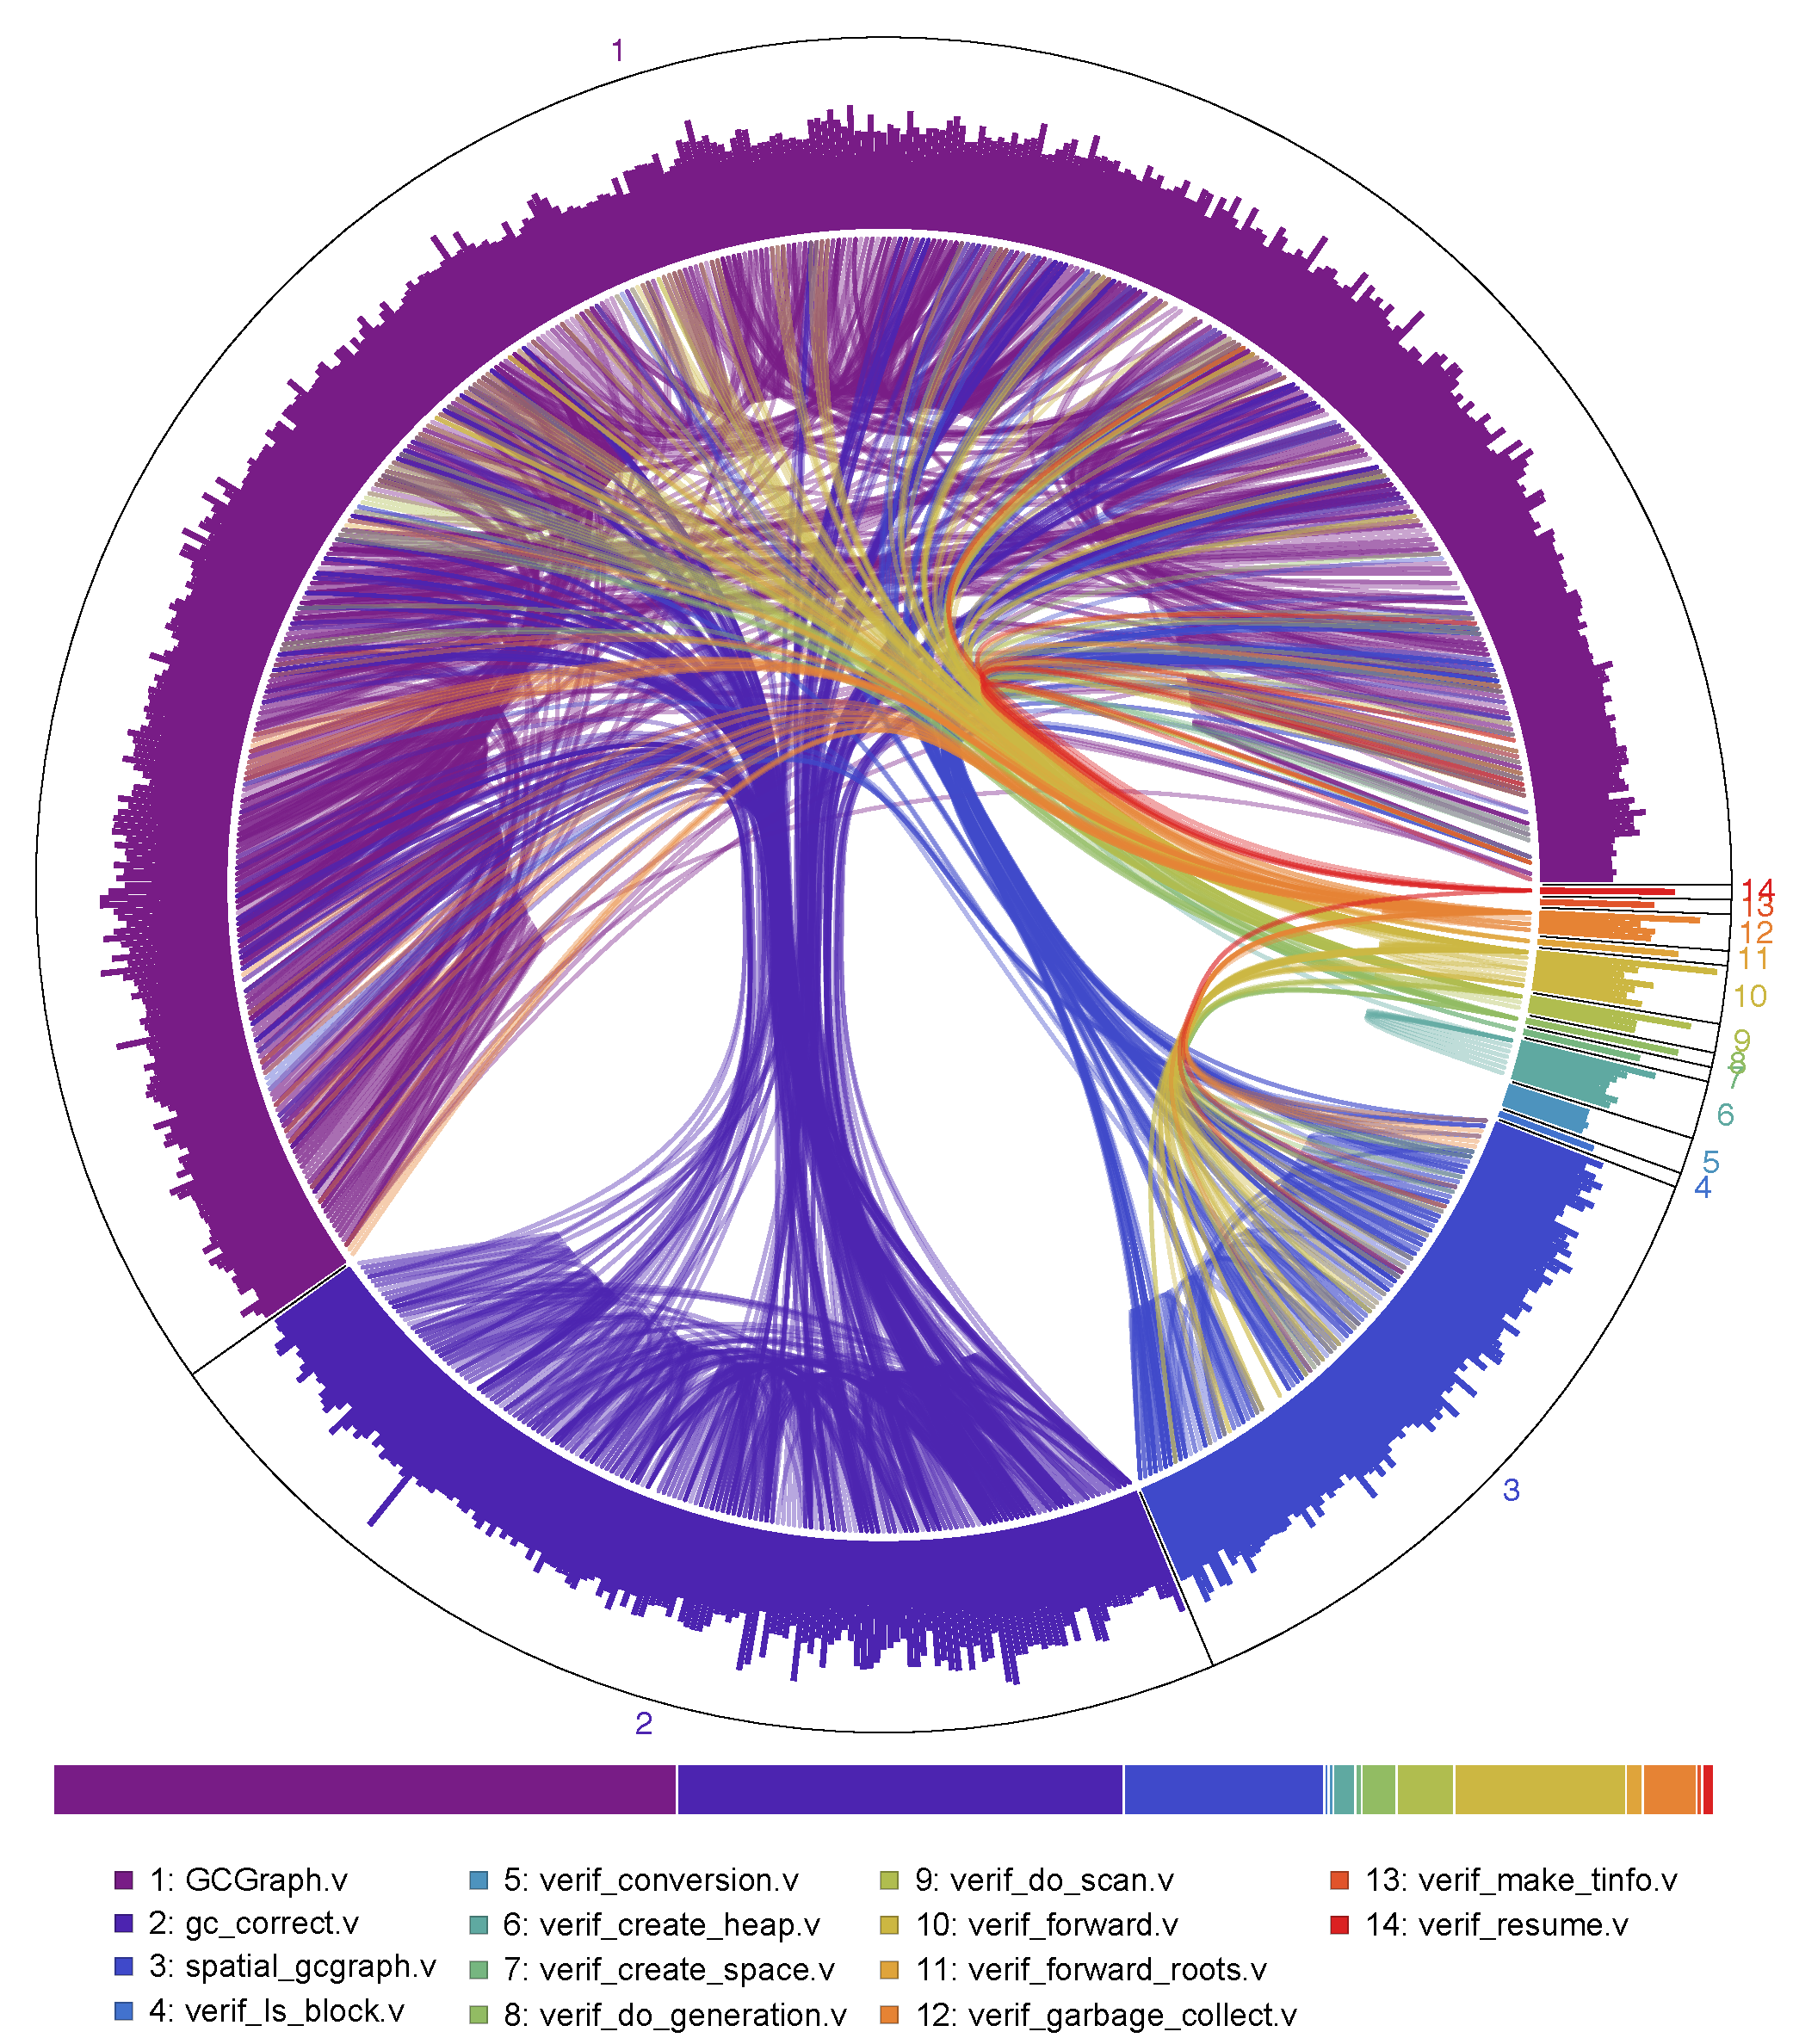
\includegraphics[width=0.95\textwidth]{certigc_theorems}
\caption{Theorems in the verification of the GC}
\label{fig:connectedness}
\end{figure}

As discussed in~\S\ref{sec:mathgraph} and~\S\ref{sec:spacegraph}, 
we made a significant effort to increase the modularity of our library and to 
encourage proof reuse.
Figure~\ref{fig:connectedness} gives a sense of this engineering effort. 
Each line in the perimeter represents a theorem used to verify the GC, 
with the length of a line corresponding to the length of the theorem on a 
logarithmic scale. The fourteen color-coded sectors represent the files in which 
these theorems are housed, and arcs connecting theorems represent dependencies. 
An arc is colored the same as the \emph{caller}.

Sector $1$ contains $432$ generic helper theorems used to check that functions
satisfy the inductive spatial relations that we need. These theorems do not depend
on any other part of the development. Sector $2$ contains $155$ theorems that 
prove the final mathematical graph isomorphism (see~\S\ref{sec:mathgraph}).
These theorems depend only on Sector $1$, 
and no other sectors depend on them. This is to be expected, seeing as graph
isomorphism is our final goal. Sector $3$ contains $91$ theorems that establish  
spatial correctness (see~\S\ref{sec:spacegraph}). Sectors $4$-$14$ are the actual
proof scripts for individual functions of the C code. Unsurprisingly, they depend
chiefly on Sectors $1$ and $3$. 



\hide{
\paragraph{Size of Coq mathgraph \S\ref{sec:mathgraph}.}
Graph folder has 18 files in total with 10,919 lines in total

\paragraph{Size of Coq spacegraph \S\ref{sec:spacegraph}.}

not including the connection to H/S or VST

include \li{Graph.v} and \li{GraphBi.v} from \li{msl_application} since they do not depend on the underlying VST model?

What is in \li{ramification_lemmas}?  %Any other parts of VST ``standard'' from our work?

\paragraph{Integration into Floyd (\S\ref{sec:vst}).}: ?
Size of additions to VST logic model: ?

\paragraph{Modifications to HIP/SLEEK.}
H/S code: approximately 2,500 lines of code across 51 files
Size of extra H/S memory model:
\li{alg_seplog_direct.v}  52 lines
\li{overlapping_direct.v} 442 lines  {\color{magenta}How do we handle alignment?}
\li{precise_direct.v} 111 lines
other files?

\paragraph{Size of VST examples~\S\ref{sec:application}.}

Note: graph, graphbi (in space), graphmark, graphbimark are shared in \li{msl_application}

mark graph  19 + 402 + 161 + 246 = 828
mark dag  19 + 402 + 161 + 210
Note: mark dag shares 19 + 402 + 161 with mark graph

copy   459 + 19 + 161 + 388 = 1,027 (need to add files from \li{msl_applicatin})
dispose   475 + 18 + 544 = 1,037 (need to add files from \li{data_structure})
What do copy or dispose share with mark or with each other?

total: 1,038 (marks) + 2,064 (copy/dispose, assuming no duplication) = 3,102 lines.  12 files, assuming no sharing for copy/dispose (with each other or with mark)

\paragraph{Size of H/S example.}
main file: 54 lines (Figure~\ref{fig:hipmarkgraph}), \li{Module Type} generated by H/S (Figure~\ref{fig:hipcoqfile}) is 30 lines, Coq \li{Module} matching this \li{Module Type} is 358 lines.
total: 2 human-generated files, 429 lines

\paragraph{Size of total development.} ?
}
